\documentclass[11pt]{beamer}
\usetheme{Singapore}
\usepackage[utf8]{inputenc}
\usepackage{verbatim}
\usepackage{amsmath}
\usepackage{amsfonts}
\usepackage{amssymb}
\usepackage{graphicx}
\usepackage{cancel}
\usepackage{verbatim}
\usepackage[backend=bibtex]{biblatex}
\addbibresource{mybib.bib}
%\setbeamertemplate{bibliography item}{\insertbiblabel}
\author{Bithiah Yuan}
\title{A Comparison of Facial Feature Extraction Methods based on Professional Domain Clustering}
%\setbeamercovered{transparent} 
%\setbeamertemplate{navigation symbols}{} 
%\logo{} 
\date{} 
\institute{\normalsize Master Project \\ University of Freiburg - Department of Compute Science \\ Chair of Databases and Information Systems} 
\setbeamertemplate{footline}[frame number]
 

\begin{document}

\begin{frame}
\titlepage
\end{frame}

\section{Introduction}

\begin{frame}{Introduction}
\begin{tabular}{l}
\parbox{1\linewidth}{
\frametitle{Motivation}
\begin{itemize}
\setlength\itemsep{1em}
\item \textbf{Question:} Can facial features predict a person's professional talents?
\item \textbf{Problem:} Research in the social sciences are limited in scalability, consistency, and generalization
\item \textbf{Solution:} Computational method based on data and face clustering
\end{itemize} }
\end{tabular}    
\end{frame}

\begin{frame}{Face Clustering}
\begin{tabular}{l}
\parbox{1\linewidth}{
\frametitle{Face Clustering}
\begin{itemize}
\setlength\itemsep{1em}
\item Clustering is an unsupervised learning technique
\item Groups data points into clusters based on their similarities \item Group similar faces together and evaluate the clusters
\item The accuracy can determine if facial features are correlated with one's professional domain
\item Face clustering is usually composed of 4 steps
\end{itemize}}
\end{tabular}  
\end{frame}

\section{Face Clustering}
\begin{frame}{Face Clustering}
\begin{tabular}{l}
\parbox{1\linewidth}{
\frametitle{Face Clustering}
\bigskip
\textbf{1. Face Detection:} Detect the position of the faces in an image and returns the coordinates of a bounding box for each face\\

\textbf{2. Face Alignment:} Find a set of facial landmarks, resize and crop the image to the edges of the landmarks
\begin{figure}[!tbp]
  \centering
  \begin{minipage}[b]{0.49\textwidth}
    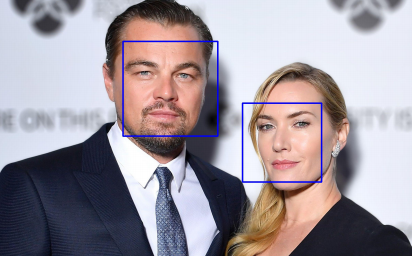
\includegraphics[width=\textwidth]{figures/face_detection.png}
    \caption{Face Detection \cite{trigueros}}
    \label{fig:detect}
  \end{minipage}
    \begin{minipage}[b]{0.49\textwidth}
    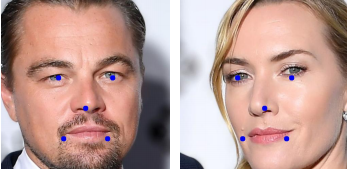
\includegraphics[width=\textwidth]{figures/landmark.png}
    \caption{Face Alignment \cite{trigueros}}
    \label{fig:landmark}
  \end{minipage}
\end{figure}
}
\end{tabular}  
\end{frame}


\begin{frame}
\frametitle{References}
\printbibliography
\end{frame}



\end{document}